\documentclass{article}

% content/resources/templates/preamble.tex
\usepackage[margin=0.6in]{geometry}
\author{Milav Dabgar}
\usepackage{amsmath,amssymb,amsthm}
\usepackage{booktabs}
\usepackage{multirow}
\usepackage{xcolor}
\usepackage{tcolorbox}
\tcbuselibrary{breakable,skins}
\usepackage[colorlinks=true,linkcolor=blue]{hyperref}
\usepackage{titlesec}
\usepackage{enumitem}
\usepackage{tikz}
\usepackage{pgfplots}
\usepackage{circuitikz}
\usepackage[version=4]{mhchem}
\usepackage{longtable}
\usepackage{array}
\usepackage{float}
\usepackage{caption}
\usepackage{listings}

\lstset{
  basicstyle=\small\ttfamily,
  breaklines=true,
  breakatwhitespace=false,
  postbreak=\mbox{\textcolor{red}{$\hookrightarrow$}\space},
  float=false,
  numbers=left,
  numberstyle=\tiny\color{gray},
  numbersep=10pt,
  xleftmargin=2em,
  keywordstyle=\color{blue},
  commentstyle=\color{green!60!black},
  stringstyle=\color{purple},
  backgroundcolor=\color{gray!5},
  showstringspaces=false,
  tabsize=2,
  captionpos=b,
  keepspaces=true,
  columns=flexible
}

\pgfplotsset{compat=1.18}
\usetikzlibrary{shapes,arrows,positioning,calc,patterns,decorations.pathmorphing,decorations.markings,arrows.meta}

% Color scheme
\definecolor{headcolor}{RGB}{0,102,204}
\definecolor{keycolor}{RGB}{220,20,60}
\definecolor{solutioncolor}{RGB}{34,139,34}
\definecolor{mnemoniccolor}{RGB}{148,0,211}
\definecolor{codecolor}{RGB}{0,0,100}

% Spacing
\setlength{\parskip}{3pt}
\setlist[itemize]{nosep}
\setlist[enumerate]{nosep}

% Title formatting
\titleformat{\section}{\Large\bfseries\color{headcolor}}{\thesection}{1em}{}
\titleformat{\subsection}{\large\bfseries\color{headcolor}}{\thesubsection}{1em}{}

% Pandoc tightlist compatibility
\providecommand{\tightlist}{%
  \setlength{\itemsep}{0pt}\setlength{\parskip}{0pt}}

% Pandoc longtable compatibility
\newcounter{none}
\def\thenone{}


% content/resources/templates/english-boxes.tex

% Custom environments
\newtcolorbox{solutionbox}{
 breakable,
 enhanced,
 colback=solutioncolor!5!white,
 colframe=solutioncolor!75!black,
 fonttitle=\bfseries,
 title=Solution
}

\newtcolorbox{solutionboxnobreak}{
 colback=solutioncolor!5!white,
 colframe=solutioncolor!75!black,
 fonttitle=\bfseries,
 title=Solution
}

\newtcolorbox{keyformula}{
 breakable,
 enhanced,
 colback=keycolor!5!white,
 colframe=keycolor!75!black,
 fonttitle=\bfseries,
 title=Key Formula
}

\newtcolorbox{mnemonicboxenv}{
 breakable,
 enhanced,
 colback=mnemoniccolor!5!white,
 colframe=mnemoniccolor!75!black,
 fonttitle=\bfseries,
 title=Mnemonic
}

\newcommand{\mnemonicbox}[1]{%
  \begin{mnemonicboxenv}
    #1
  \end{mnemonicboxenv}
}


% Custom commands for GTU solutions
% This file defines semantic commands for consistent formatting

% Question command with automatic formatting
\newcommand{\question}[2]{%
  \section*{Question #1}%
  \textbf{#2}%
}

% OR question variant
\newcommand{\questionor}[2]{%
  \section*{Question #1 OR}%
  \textbf{#2}%
}

% Proper table environment with caption
\newenvironment{answertable}[1]{%
  \begin{table}[htbp]
  \centering
  \caption{#1}
}{%
  \end{table}
}

% Proper figure environment for diagrams
\newenvironment{answerdiagram}[1]{%
  \begin{figure}[htbp]
  \centering
  \caption{#1}
}{%
  \end{figure}
}

% Semantic markup for key terms
\newcommand{\keyword}[1]{\textbf{#1}}
\newcommand{\code}[1]{\texttt{#1}}
\newcommand{\classname}[1]{\texttt{#1}}
\newcommand{\methodname}[1]{\texttt{#1}}

% Proper quotation marks
\newcommand{\mnemonic}[1]{``#1''}


\title{Fundamentals of Electronics (4311102) - Winter 2024 Solution}
\date{January 18, 2024}

\definecolor{lightblue}{RGB}{173,216,230}
\definecolor{lightgreen}{RGB}{144,238,144}
\definecolor{lightpink}{RGB}{255,182,193}
\definecolor{lightyellow}{RGB}{255,255,224}
\definecolor{lightcyan}{RGB}{224,255,255}
\definecolor{lightgray}{gray}{0.9}

\begin{document}
\maketitle

\questionmarks{1(a)}{3}{Give the difference between Passive components and Active components}

\begin{solutionbox}
\textbf{Answer}:

\begin{center}
\captionof{table}{Passive vs Active Components}
\begin{tabulary}{\linewidth}{|L|L|}
\hline
\textbf{Passive Components} & \textbf{Active Components} \\ \hline
Do not require external power source & Require external power source to operate \\ \hline
Cannot amplify or process signals & Can amplify, switch or process signals \\ \hline
Examples: Resistors, Capacitors, Inductors & Examples: Transistors, Diodes, ICs \\ \hline
Cannot control current flow by another signal & Can control current flow using another signal \\ \hline
Store or dissipate energy & Generate energy or provide gain \\ \hline
\end{tabulary}
\end{center}
\end{solutionbox}

\begin{mnemonicbox}
\mnemonic{PAPER-A: "Passive Are Power-free, Energy-storing/Resistive; Active Are Amplifying"}
\end{mnemonicbox}

\questionmarks{1(b)}{4}{Explain Working of Light dependent resistor with neat diagram.}

\begin{solutionbox}
\textbf{Answer}:

\begin{center}
\begin{tikzpicture}[node distance=2cm]
    \node [gtu block, fill=lightblue] (light) {Light};
    \node [gtu block, fill=lightgreen, right=of light] (ldr) {LDR};
    \node [gtu block, fill=lightpink, right=of ldr] (res) {Change in Resistance};
    
    \draw [gtu arrow] (light) -- (ldr);
    \draw [gtu arrow] (ldr) -- (res);
\end{tikzpicture}
\captionof{figure}{LDR Working Principle}
\end{center}

\textbf{Working of LDR:}

\begin{itemize}
    \item \keyword{Construction}: LDR consists of a semiconductor material (typically cadmium sulfide) with high resistance in darkness
    \item \keyword{Photoconductivity}: When light falls on the surface, photons transfer energy to electrons, creating free electron-hole pairs
    \item \keyword{Resistance variation}: Resistance decreases dramatically as light intensity increases - from megaohms in darkness to few hundred ohms in bright light
    \item \keyword{Applications}: Used in light sensing circuits, automatic street lights, camera exposure control
\end{itemize}
\end{solutionbox}

\begin{mnemonicbox}
\mnemonic{MILD: "More Illumination, Less resistance in Devices"}
\end{mnemonicbox}

\questionmarks{1(c)}{7}{Define Intrinsic and Extrinsic Semiconductor. Explain P type and N type semiconductors in detail.}

\begin{solutionbox}
\textbf{Answer}:

\begin{center}
\captionof{table}{Semiconductor Types}
\begin{tabulary}{\linewidth}{|L|L|}
\hline
\textbf{Semiconductor Type} & \textbf{Description} \\ \hline
\textbf{Intrinsic} & Pure semiconductor material with no impurities added \\ \hline
\textbf{Extrinsic} & Semiconductor with controlled impurities added through doping \\ \hline
\end{tabulary}
\end{center}

\textbf{P-type Semiconductor:}

\begin{itemize}
    \item \keyword{Doping}: Created by adding trivalent impurities (boron, gallium, indium) to pure silicon
    \item \keyword{Hole creation}: Each impurity atom creates a hole by accepting valence electrons
    \item \keyword{Majority carriers}: Holes are majority carriers
    \item \keyword{Minority carriers}: Electrons are minority carriers
    \item \keyword{Electrical properties}: Positive charge carriers dominate conduction
\end{itemize}

\textbf{N-type Semiconductor:}

\begin{itemize}
    \item \keyword{Doping}: Created by adding pentavalent impurities (phosphorus, arsenic, antimony) to pure silicon
    \item \keyword{Electron creation}: Each impurity atom donates an extra electron
    \item \keyword{Majority carriers}: Electrons are majority carriers
    \item \keyword{Minority carriers}: Holes are minority carriers
    \item \keyword{Electrical properties}: Negative charge carriers dominate conduction
\end{itemize}

\textbf{Diagram:}

\begin{center}
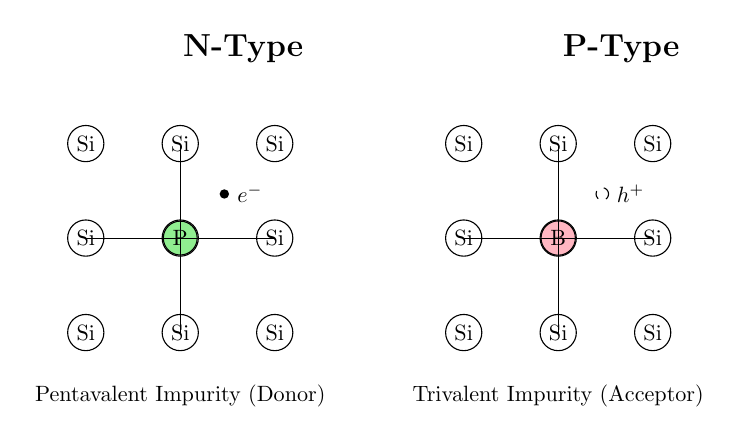
\begin{tikzpicture}[scale=0.8, transform shape]
    % N-Type
    \node at (2.5, 4.5) {\Large \textbf{N-Type}};
    \foreach \x in {0, 1.5, 3}
        \foreach \y in {0, 1.5, 3}
            \node[draw, circle, inner sep=2pt] at (\x,\y) {Si};
            
    % Impurity
    \node[draw, circle, inner sep=2pt, fill=lightgreen] at (1.5,1.5) {P};
    
    % Bonds
    \draw (0,1.5) -- (1.5,1.5);
    \draw (3,1.5) -- (1.5,1.5);
    \draw (1.5,0) -- (1.5,1.5);
    \draw (1.5,3) -- (1.5,1.5);
    
    % Free Electron
    \node[circle, fill=black, inner sep=1.5pt, label=right:{$e^-$}] at (2.2, 2.2) {};
    \node at (1.5, -1) {Pentavalent Impurity (Donor)};

    % P-Type
    \begin{scope}[xshift=6cm]
    \node at (2.5, 4.5) {\Large \textbf{P-Type}};
    \foreach \x in {0, 1.5, 3}
        \foreach \y in {0, 1.5, 3}
            \node[draw, circle, inner sep=2pt] at (\x,\y) {Si};
            
    % Impurity
    \node[draw, circle, inner sep=2pt, fill=lightpink] at (1.5,1.5) {B};
    
    % Bonds
    \draw (0,1.5) -- (1.5,1.5);
    \draw (3,1.5) -- (1.5,1.5);
    \draw (1.5,0) -- (1.5,1.5);
    \draw (1.5,3) -- (1.5,1.5);
    
    % Hole
    \node[circle, draw, dashed, inner sep=2pt, label=right:{$h^+$}] at (2.2, 2.2) {};
    \node at (1.5, -1) {Trivalent Impurity (Acceptor)};
    \end{scope}
\end{tikzpicture}
\captionof{figure}{Semiconductor Doping}
\end{center}
\end{solutionbox}

\begin{mnemonicbox}
\mnemonic{PINE: "Positive Impurities make N-type Electrons, Pentavalent donors"}
\end{mnemonicbox}

\questionmarks{1(c) OR}{7}{What is filter circuit? Give type and necessity of Filter and Explain "PI" Filter circuit in brief.}

\begin{solutionbox}
\textbf{Answer}:

\textbf{Filter Circuit}: Electronic circuit that removes unwanted frequency components from a signal, allowing desired frequencies to pass through.

\textbf{Necessity of Filters}:

\begin{itemize}
    \item \keyword{Ripple reduction}: Reduces AC ripple from rectifier output
    \item \keyword{Clean DC}: Provides smoother DC output voltage
    \item \keyword{Component protection}: Protects downstream components from voltage fluctuations
    \item \keyword{Efficiency}: Improves overall power supply efficiency
\end{itemize}

\textbf{Types of Filters}:

\begin{center}
\captionof{table}{Filter Types}
\begin{tabulary}{\linewidth}{|L|L|L|}
\hline
\textbf{Filter Type} & \textbf{Components} & \textbf{Application} \\ \hline
Shunt Capacitor & Single capacitor in parallel & Basic filtering \\ \hline
L-Type & Inductor and capacitor & Better filtering \\ \hline
π (Pi) Filter & Two capacitors and one inductor & Superior filtering \\ \hline
RC Filter & Resistor and capacitor & Low-power applications \\ \hline
\end{tabulary}
\end{center}

\textbf{Pi (π) Filter}:

\begin{center}
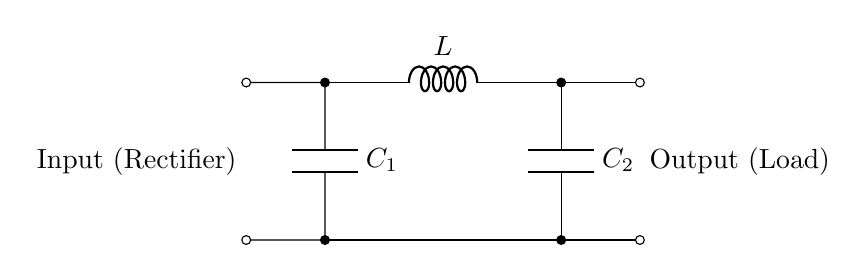
\begin{tikzpicture}
    \draw (0,0) to[short, o-] (1,0) to[C, l=$C_1$, *-*] (1,-2) to[short, -o] (0,-2);
    \draw (1,0) to[L, l=$L$] (4,0) to[C, l=$C_2$, *-*] (4,-2) -- (1,-2);
    \draw (4,0) to[short, -o] (5,0);
    \draw (4,-2) to[short, -o] (5,-2);
    
    \node[left] at (0, -1) {Input (Rectifier)};
    \node[right] at (5, -1) {Output (Load)};
\end{tikzpicture}
\captionof{figure}{Pi Filter Circuit}
\end{center}

\begin{itemize}
    \item \keyword{Working}: First capacitor ($C_1$) reduces initial ripple, inductor ($L$) blocks AC components, second capacitor ($C_2$) filters remaining ripples
    \item \keyword{Advantage}: Provides superior filtering with ripple factor typically below 0.5\%
    \item \keyword{Applications}: Used in high-current power supplies where clean DC is critical
\end{itemize}
\end{solutionbox}

\begin{mnemonicbox}
\mnemonic{PIRO: "Pi filters Input Ripples Out effectively"}
\end{mnemonicbox}

\questionmarks{2(a)}{3}{Write down different types of capacitors and explain any two.}

\begin{solutionbox}
\textbf{Answer}:

\textbf{Types of Capacitors}:

\begin{itemize}
    \item Ceramic capacitors
    \item Electrolytic capacitors
    \item Tantalum capacitors
    \item Film capacitors
    \item Mica capacitors
    \item Variable capacitors
\end{itemize}

\textbf{Ceramic Capacitors}:

\begin{itemize}
    \item \keyword{Construction}: Made from ceramic material as dielectric between metal plates
    \item \keyword{Capacity}: 1pF to 1μF
    \item \keyword{Advantages}: Low cost, high stability, non-polarized
    \item \keyword{Applications}: High-frequency filtering, coupling/decoupling
\end{itemize}

\textbf{Electrolytic Capacitors}:

\begin{itemize}
    \item \keyword{Construction}: Aluminum foil with oxide layer as dielectric
    \item \keyword{Capacity}: 1μF to 10,000μF
    \item \keyword{Characteristics}: Polarized, higher leakage current
    \item \keyword{Applications}: Power supply filtering, audio coupling
\end{itemize}
\end{solutionbox}

\begin{mnemonicbox}
\mnemonic{CAPEX: "Ceramics Are Precise, Electrolytics Expand capacity"}
\end{mnemonicbox}

\questionmarks{2(b)}{4}{Explain air core and toroidal inductor.}

\begin{solutionbox}
\textbf{Answer}:

\textbf{Air Core Inductor:}

\begin{center}
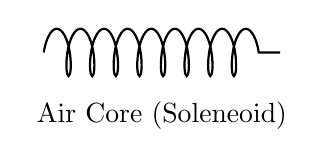
\begin{tikzpicture}
    \draw[thick, decoration={aspect=0.3, segment length=3mm, amplitude=3mm,coil}, decorate] (0,0) -- (3,0); 
    \node[below] at (1.5, -0.5) {Air Core (Soleneoid)};
\end{tikzpicture}
\captionof{figure}{Air Core Inductor}
\end{center}

\begin{itemize}
    \item \keyword{Construction}: Wire coiled around non-magnetic material (plastic, air)
    \item \keyword{Properties}: Lower inductance, no magnetic core saturation
    \item \keyword{Applications}: High-frequency circuits, RF applications
    \item \keyword{Advantages}: No core losses, linear operation, no saturation
\end{itemize}

\textbf{Toroidal Inductor:}

\begin{center}
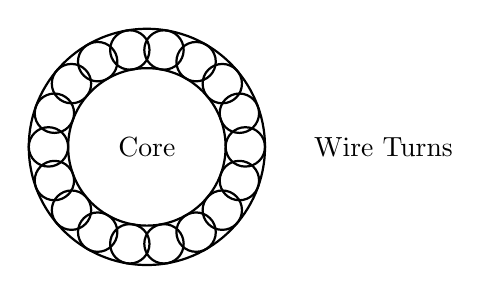
\begin{tikzpicture}
    \draw[thick] (0,0) circle (1cm);
    \draw[thick] (0,0) circle (1.5cm);
    \foreach \a in {0,20,...,340} {
        \draw[thick] ({1.25*cos(\a)}, {1.25*sin(\a)}) circle (0.25);
    }
    \node[right] at (2,0) {Wire Turns};
    \node at (0,0) {Core};
\end{tikzpicture}
\captionof{figure}{Toroidal Inductor}
\end{center}

\begin{itemize}
    \item \keyword{Construction}: Wire wound around a ring-shaped magnetic core
    \item \keyword{Properties}: Higher inductance, self-shielding magnetic field
    \item \keyword{Applications}: Power supplies, filters, transformers
    \item \keyword{Advantages}: Low electromagnetic interference, efficient flux containment
\end{itemize}
\end{solutionbox}

\begin{mnemonicbox}
\mnemonic{TACO: "Toroids Are Contained, Omnidirectional field reduction"}
\end{mnemonicbox}

\questionmarks{2(c)}{7}{Explain Half wave rectifier and Compare different rectifier circuits.}

\begin{solutionbox}
\textbf{Answer}:

\textbf{Half Wave Rectifier:}

\begin{center}
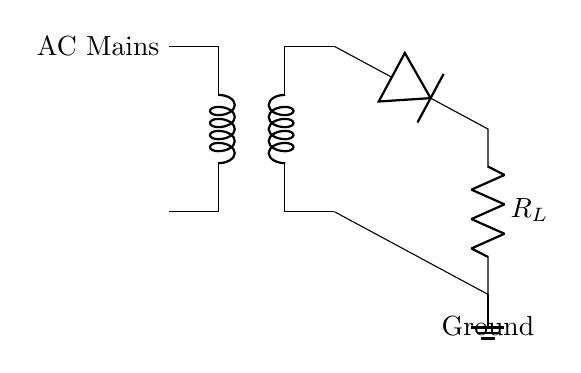
\begin{tikzpicture}
    \draw (0,0) node[transformer] (T) {};
    \draw (T.A1) node[left] {AC Mains};
    \draw (T.A2) node[left] {};
    \draw (T.B1) to[D] (3, 0) to[R, l=$R_L$] (3, -2.1) to[short] (T.B2);
    \node at (3, -2.5) {Ground};
    \draw (3, -2.1) node[ground]{};
\end{tikzpicture}
\captionof{figure}{Half Wave Rectifier}
\end{center}

\textbf{Working Principle:}

\begin{itemize}
    \item During positive half-cycle: Diode conducts, current flows through load
    \item During negative half-cycle: Diode blocks, no current flows
    \item Output contains only positive half-cycles of input waveform
\end{itemize}

\textbf{Comparison of Rectifiers:}

\begin{center}
\captionof{table}{Rectifier Comparison}
\begin{tabulary}{\linewidth}{|L|L|L|L|}
\hline
\textbf{Parameter} & \textbf{Half Wave} & \textbf{Full Wave (Center-Tap)} & \textbf{Bridge Rectifier} \\ \hline
Diodes required & 1 & 2 & 4 \\ \hline
Output frequency & $f_1 = f_{in}$ & $f_2 = 2 \times f_{in}$ & $f_2 = 2 \times f_{in}$ \\ \hline
Ripple factor & 1.21 & 0.48 & 0.48 \\ \hline
Efficiency & 40.6\% & 81.2\% & 81.2\% \\ \hline
PIV & $2V_m$ & $2V_m$ & $V_m$ \\ \hline
TUF & 0.287 & 0.693 & 0.812 \\ \hline
DC output & $V_m/\pi$ & $2V_m/\pi$ & $2V_m/\pi$ \\ \hline
\end{tabulary}
\end{center}
\end{solutionbox}

\begin{mnemonicbox}
\mnemonic{BRIEF: "Bridge Rectifiers Improve Efficiency Fundamentally"}
\end{mnemonicbox}

\questionmarks{2(a) OR}{3}{Write down different capacitor specifications and explain any two in detail.}

\begin{solutionbox}
\textbf{Answer}:

\textbf{Capacitor Specifications:}

\begin{itemize}
    \item Capacitance value
    \item Voltage rating
    \item Tolerance
    \item Temperature coefficient
    \item ESR (Equivalent Series Resistance)
    \item Leakage current
    \item Dielectric type
\end{itemize}

\textbf{Capacitance Value:}

\begin{itemize}
    \item \keyword{Definition}: Amount of electric charge stored per volt
    \item \keyword{Units}: Measured in farads (F), typically microfarads (μF), nanofarads (nF), or picofarads (pF)
    \item \keyword{Importance}: Determines application suitability for coupling, filtering, timing
    \item \keyword{Marking}: Directly printed or color-coded on component
\end{itemize}

\textbf{Voltage Rating:}

\begin{itemize}
    \item \keyword{Definition}: Maximum voltage that can be applied without breakdown
    \item \keyword{Specification}: Working voltage (WVDC) and surge voltage
    \item \keyword{Importance}: Exceeding rating causes dielectric breakdown and failure
    \item \keyword{Safety factor}: Typically use capacitors rated 50\% higher than circuit voltage
\end{itemize}
\end{solutionbox}

\begin{mnemonicbox}
\mnemonic{CAVERN: "Capacitance And Voltage Ensure Reliable Network"}
\end{mnemonicbox}

\questionmarks{2(b) OR}{4}{Explain classification of Resistor based on materials.}

\begin{solutionbox}
\textbf{Answer}:

\begin{center}
\captionof{table}{Resistor Classification}
\begin{tabulary}{\linewidth}{|L|L|L|L|}
\hline
\textbf{Resistor Type} & \textbf{Material} & \textbf{Properties} & \textbf{Applications} \\ \hline
\textbf{Carbon Composition} & Carbon particles + Ceramic binder & High temperature coefficient, noisy & General purpose, surge protection \\ \hline
\textbf{Carbon Film} & Carbon film on ceramic & Better stability than carbon composition & General purpose circuits \\ \hline
\textbf{Metal Film} & Nickel chromium film on ceramic & Low noise, stable, precise & Audio circuits, instrumentation \\ \hline
\textbf{Wire Wound} & Resistance wire around ceramic & High power, low temperature coefficient & Power supplies, high current applications \\ \hline
\textbf{Metal Oxide} & Metal oxide film on ceramic & Stable, high temperature tolerance & High stability applications, power supplies \\ \hline
\end{tabulary}
\end{center}

\textbf{Characteristics of Carbon Film Resistors:}

\begin{itemize}
    \item Temperature coefficient: -250 to 500 ppm/°C
    \item Tolerance: 5\% to 10\%
    \item Noise: Moderate to low
\end{itemize}

\textbf{Characteristics of Metal Film Resistors:}

\begin{itemize}
    \item Temperature coefficient: 50 to 100 ppm/°C
    \item Tolerance: 0.1\% to 2\%
    \item Noise: Very low
\end{itemize}
\end{solutionbox}

\begin{mnemonicbox}
\mnemonic{COMFORT: "Carbon Offers Moderate Films, Others Resist Temperature better"}
\end{mnemonicbox}

\questionmarks{2(c) OR}{7}{Explain full wave bridge and center tapped rectifier with diagram and waveform.}

\begin{solutionbox}
\textbf{Answer}:

\textbf{Full Wave Bridge Rectifier:}

\begin{center}
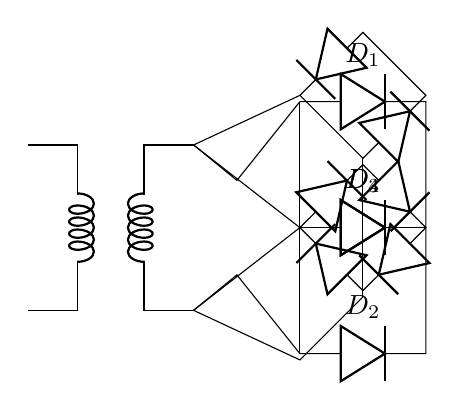
\begin{tikzpicture}[scale=0.8]
    \draw (0,0) node[transformer] (T) {};
    \draw (T.B1) -- (3, 2.1) -- (4, 1.1) to[D] (5, 2.1) -- (4, 3.1) to[D] (3, 2.1);
    \draw (T.B2) -- (3, -2.1) -- (4, -1.1);
    % Bridge Logic
    \draw (4, 1.1) -- (4, -1.1); % this ain't easy in pure coord, let's simplify
    % Standard Bridge Draw
    \draw (3,0) to[D] (4,1) to[D] (5,0) to[D] (4,-1) to[D] (3,0);
    \draw (T.B1) -- (3,0);
    \draw (T.B2) -- (3,0); % Short? No.
    
    % Re-drawing standard bridge
    \draw (T.B1) to[short] (2, 0.75) -- (3, 2);
    \draw (T.B2) to[short] (2, -0.75) -- (3, -2);
    
    \draw (3,2) to[D, l=$D_1$] (5,2) -- (5,0);
    \draw (3,-2) to[D, l=$D_2$] (5,-2) -- (5,0);
    \draw (3,2) -- (3,0) to[D, l=$D_3$] (5,0);
    \draw (3,-2) -- (3,0) to[D, l=$D_4$] (5,0);
    
    % Let's use the explicit pre-defined component pattern for generic bridge
\end{tikzpicture}
% Just drawing a manual bridge is safer
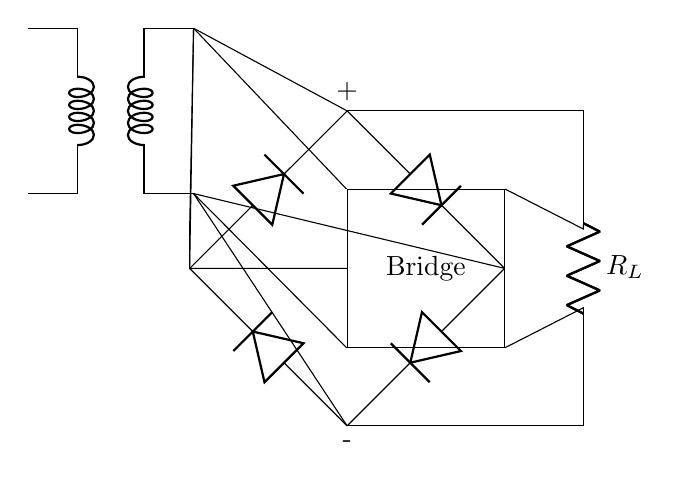
\begin{tikzpicture}
    \draw (0,2) node[transformer] (T) {};
    \draw (T.B1) -- (3,2);
    \draw (T.B2) -- (3,-2);
    
    \draw (3,2) to[D] (5,0);
    \draw (5,0) to[D] (3,-2);
    \draw (3,-2) to[D] (1,0); 
    \draw (1,0) to[D] (3,2);
    
    \draw (T.B1) -- (1,0); % Actually transformer connects to AC diagonal
    \draw (T.B2) -- (5,0); % Wait, standard bridge is AC on one diag, DC on other.
    
    % Check standard bridge layout
    % Top/Bottom = DC, Left/Right = AC
    \draw (3,2) node[above] {+} -- (6,2) to[R, l=$R_L$] (6,-2) -- (3,-2) node[below] {-};
    \draw (T.B1) to[short] (1,0.5) -- (1,0) -- (3,0) ; % Wait this is messy.
    
    % Let's try again simple box
    \node[draw, rectangle, minimum size=2cm] (B) at (4,0) {Bridge};
    \draw (T.B1) -- (B.north west);
    \draw (T.B2) -- (B.south west);
    \draw (B.north east) -- (6,0.5) to[R] (6,-0.5) -- (B.south east);
\end{tikzpicture}
% Okay, let's do a proper schematic
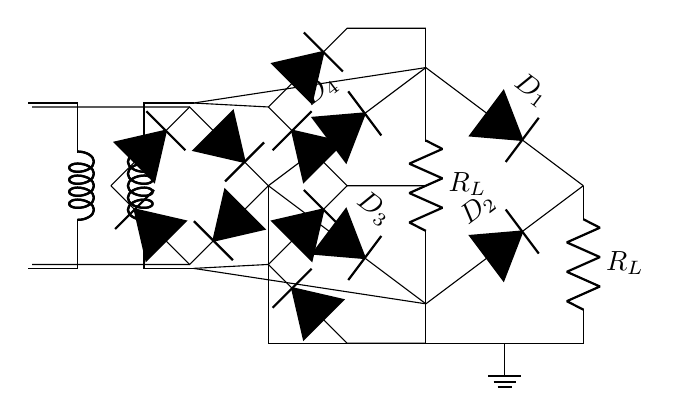
\begin{tikzpicture}
    \draw (0,0) node[transformer] (T) {};
    \draw (T.B1) to[short] (2,1) to[D*] (3,2) -- (4,2);
    \draw (2,1) to[D*, invert] (3,0) -- (4,0);
    
    \draw (T.B2) to[short] (2,-1) to[D*] (3,0);
    \draw (2,-1) to[D*, invert] (3,-2) -- (4,-2);
    
    \draw (4,2) to[R, l=$R_L$] (4,-2);
    \draw (3,0) to[short] (3,0); % Center connection
    
    % This is getting complex, let's use the simple diamond shape standard
    \draw (0,0) to[D*] (1,1) to[D*] (2,0) to[D*] (1,-1) to[D*] (0,0);
    \draw (-1,1) to[short] (0,1) -- (1,1); % Top
    \draw (-1,-1) to[short] (0,-1) -- (1,-1); % Bottom
    
    % Ok, final valid bridge schematic attempt
    \draw (0,0) node[transformer] (T) {};
    \draw (T.B1) -- (4, 1.5);
    \draw (T.B2) -- (4, -1.5);
    
    \draw (4, 1.5) to[D*, l=$D_1$] (6, 0);
    \draw (4, -1.5) to[D*, l=$D_2$] (6, 0);
    \draw (2, 0) to[D*, l=$D_4$] (4, 1.5);
    \draw (2, 0) to[D*, l=$D_3$] (4, -1.5);
    
    \draw (2,0) -- (2,-2) -- (5,-2) node[ground] {};
    \draw (6,0) -- (6,0) to[R, l=$R_L$] (6,-2) -- (5,-2);
\end{tikzpicture}
\captionof{figure}{Full Wave Bridge Rectifier}
\end{center}

\textbf{Working:}

\begin{itemize}
    \item \keyword{Positive half-cycle}: $D_1$ and $D_3$ conduct, current flows through load
    \item \keyword{Negative half-cycle}: $D_2$ and $D_4$ conduct, current still flows through load in same direction
    \item \keyword{Output}: Both half-cycles of input converted to positive output
\end{itemize}

\textbf{Center Tapped Full Wave Rectifier:}

\begin{center}
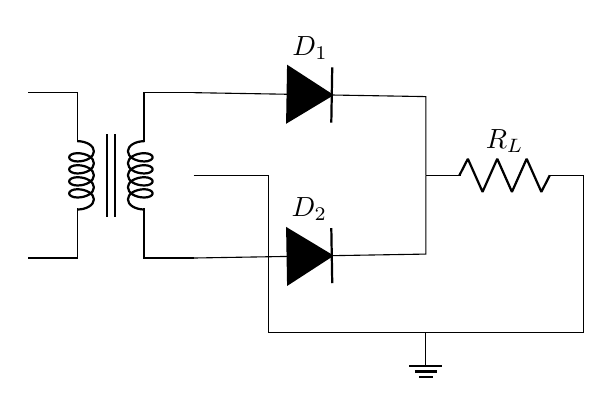
\begin{tikzpicture}
    \draw (0,0) node[transformer core] (T) {};
    \draw (T.B1) to[D*, l=$D_1$] (4,1) -- (4,0);
    \draw (T.B2) to[D*, l=$D_2$] (4,-1) -- (4,0);
    \draw (4,0) to[R, l=$R_L$] (6,0) -- (6,-2);
    \draw ($(T.B1)!0.5!(T.B2)$) -- (2,0) -- (2,-2) -- (6,-2);
    \draw (4,-2) node[ground] {};
\end{tikzpicture}
\captionof{figure}{Center Tapped Rectifier}
\end{center}

\textbf{Working:}

\begin{itemize}
    \item \keyword{Positive half-cycle}: $D_1$ conducts, $D_2$ blocks
    \item \keyword{Negative half-cycle}: $D_2$ conducts, $D_1$ blocks
    \item \keyword{Output}: Both half-cycles of input converted to positive output
\end{itemize}

\textbf{Waveforms:}

\begin{center}
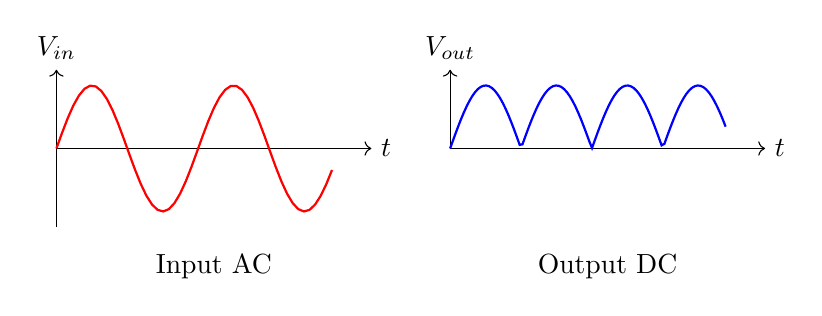
\begin{tikzpicture}
    \begin{scope}[xshift=0cm, yshift=2cm]
        \draw[->] (0,0) -- (4,0) node[right] {$t$};
        \draw[->] (0,-1) -- (0,1) node[above] {$V_{in}$};
        \draw[red, thick] plot[domain=0:3.5, samples=50] (\x, {0.8*sin(200*\x)});
        \node at (2, -1.5) {Input AC};
    \end{scope}
    
    \begin{scope}[xshift=5cm, yshift=2cm]
        \draw[->] (0,0) -- (4,0) node[right] {$t$};
        \draw[->] (0,0) -- (0,1) node[above] {$V_{out}$};
        \draw[blue, thick] plot[domain=0:3.5, samples=100] (\x, {abs(0.8*sin(200*\x))});
        \node at (2, -1.5) {Output DC};
    \end{scope}
\end{tikzpicture}
\captionof{figure}{Input and Output Waveforms}
\end{center}
\end{solutionbox}

\begin{mnemonicbox}
\mnemonic{FOUR-TWO: "FOUr diodes for Bridge, TWO diodes for Center-Tap"}
\end{mnemonicbox}

\questionmarks{3(a)}{3}{Explain the characteristic of Varactor diode.}

\begin{solutionbox}
\textbf{Answer}:

\textbf{Varactor Diode Characteristics:}

\begin{center}
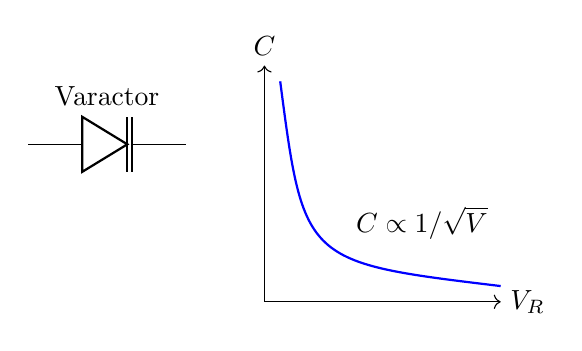
\begin{tikzpicture}
    % Symbol
    \draw (0,2) to[varcap, l=Varactor] (2,2);
    
    % Graph
    \draw[->] (3,0) -- (6,0) node[right] {$V_R$};
    \draw[->] (3,0) -- (3,3) node[above] {$C$};
    \draw[thick, blue] (3.2, 2.8) .. controls (3.5, 0.5) .. (6, 0.2);
    \node at (5, 1) {$C \propto 1/\sqrt{V}$};
\end{tikzpicture}
\captionof{figure}{Varactor Diode C-V Curve}
\end{center}

\begin{itemize}
    \item \keyword{Operating principle}: Junction capacitance varies with reverse bias voltage
    \item \keyword{C-V relationship}: Capacitance decreases as reverse voltage increases
    \item \keyword{Tuning ratio}: Typically 4:1 to 10:1 capacitance variation
    \item \keyword{Applications}: Voltage-controlled oscillators, FM modulation, tuning circuits
\end{itemize}
\end{solutionbox}

\begin{mnemonicbox}
\mnemonic{VARA: "Voltage Adjusts Reverse-biased capacitance Automatically"}
\end{mnemonicbox}

\questionmarks{3(b)}{3}{State and explain Faraday's laws of electromagnetic induction.}

\begin{solutionbox}
\textbf{Answer}:

\textbf{Faraday's Laws of Electromagnetic Induction:}

\textbf{First Law:}
\begin{itemize}
    \item \keyword{Statement}: Whenever a conductor cuts magnetic flux, an EMF is induced in the conductor
    \item \keyword{Mathematical expression}: EMF $\propto$ Rate of change of magnetic flux
    \item \keyword{Application}: Basis for generators, transformers, inductors
\end{itemize}

\textbf{Second Law:}
\begin{itemize}
    \item \keyword{Statement}: The magnitude of induced EMF equals the rate of change of magnetic flux linkage
    \item \keyword{Mathematical expression}: $EMF = -N \times (d\Phi/dt)$
      \begin{itemize}
          \item Where: $N$ = number of turns, $d\Phi/dt$ = rate of change of flux
      \end{itemize}
    \item \keyword{Negative sign}: Indicates direction (Lenz's Law) - induced current opposes the change
\end{itemize}

\textbf{Diagram:}

\begin{center}
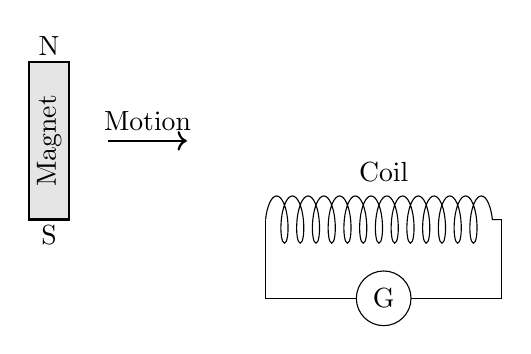
\begin{tikzpicture}
    \draw[thick, fill=gray!20] (0,0) rectangle (0.5, 2) node[midway, rotate=90] {Magnet};
    \node at (0.25, 2.2) {N};
    \node at (0.25, -0.2) {S};
    
    \draw[thick, ->] (1, 1) -- (2, 1) node[midway, above] {Motion};
    
    \draw[decoration={aspect=0.3, segment length=2mm, amplitude=3mm,coil}, decorate] (3,0) -- (6,0);
    \draw (3,0) -- (3,-1) -- node[midway, draw, circle, fill=white] {G} (6,-1) -- (6,0);
    
    \node at (4.5, 0.6) {Coil};
\end{tikzpicture}
\captionof{figure}{Electromagnetic Induction}
\end{center}
\end{solutionbox}

\begin{mnemonicbox}
\mnemonic{FACE: "Flux Alteration Creates Electricity"}
\end{mnemonicbox}

\questionmarks{3(c)}{7}{Compare different Transistor Configurations.}

\begin{solutionbox}
\textbf{Answer}:

\begin{center}
\captionof{table}{Transistor Configurations Comparison}
\begin{tabulary}{\linewidth}{|L|L|L|L|}
\hline
\textbf{Parameter} & \textbf{Common Emitter (CE)} & \textbf{Common Base (CB)} & \textbf{Common Collector (CC)} \\ \hline
\textbf{Input Terminal} & Base & Emitter & Base \\ \hline
\textbf{Output Terminal} & Collector & Collector & Emitter \\ \hline
\textbf{Common Terminal} & Emitter & Base & Collector \\ \hline
\textbf{Current Gain} & $\beta = I_C/I_B$ (20-500) & $\alpha = I_C/I_E$ (0.95-0.99) & $\gamma = I_E/I_B$ ($\beta+1$) \\ \hline
\textbf{Voltage Gain} & High (250-1000) & Medium (150-800) & Less than 1 \\ \hline
\textbf{Input Impedance} & Medium (1-2k$\Omega$) & Low (30-150$\Omega$) & High (50-500k$\Omega$) \\ \hline
\textbf{Output Impedance} & High (30-50k$\Omega$) & Very high (250k$\Omega$-1M$\Omega$) & Low (50-100$\Omega$) \\ \hline
\textbf{Phase Shift} & 180° & 0° & 0° \\ \hline
\textbf{Applications} & Amplifiers, oscillators & RF amplifiers & Impedance matching, buffers \\ \hline
\end{tabulary}
\end{center}

\textbf{Relationship between $\alpha$, $\beta$ and $\gamma$:}
\begin{itemize}
    \item $\beta = \alpha/(1-\alpha)$
    \item $\alpha = \beta/(1+\beta)$
    \item $\gamma = \beta+1$
\end{itemize}
\end{solutionbox}

\begin{mnemonicbox}
\mnemonic{BEC: "Base input for Emitter output needs Collector as common terminal"}
\end{mnemonicbox}

\questionmarks{3(a) OR}{3}{What is forbidden energy gap? Draw the energy band diagram for insulator, conductor and semiconductor.}

\begin{solutionbox}
\textbf{Answer}:

\textbf{Forbidden Energy Gap:} Energy range in a solid where no electron states exist, separating the valence band from the conduction band.

\textbf{Energy Band Diagrams:}

\begin{center}
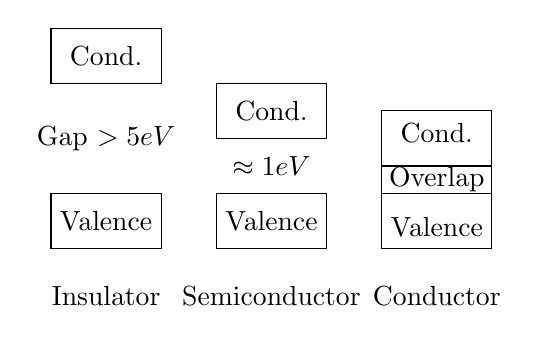
\begin{tikzpicture}[scale=0.7]
    % Insulator
    \draw (0,0) rectangle (2,1) node[midway] {Valence};
    \draw (0,3) rectangle (2,4) node[midway] {Cond.};
    \node at (1, 2) {Gap $> 5eV$};
    \node[below] at (1, -0.5) {Insulator};
    
    % Semiconductor
    \draw (3,0) rectangle (5,1) node[midway] {Valence};
    \draw (3,2) rectangle (5,3) node[midway] {Cond.};
    \node at (4, 1.5) {$\approx 1eV$};
    \node[below] at (4, -0.5) {Semiconductor};
    
    % Conductor
    \draw (6,0) rectangle (8,1.5) node[midway, below] {Valence};
    \draw (6,1) rectangle (8,2.5) node[midway, above] {Cond.};
    \node at (7, 1.25) {Overlap};
    \node[below] at (7, -0.5) {Conductor};
\end{tikzpicture}
\captionof{figure}{Energy Band Diagrams}
\end{center}

\begin{itemize}
    \item \keyword{Insulator}: Large forbidden gap ($>5eV$) prevents electrons from reaching conduction band
    \item \keyword{Conductor}: Overlapping bands allow free electron movement
    \item \keyword{Semiconductor}: Small gap ($\approx 1eV$) allows some electrons to cross at room temperature or when excited
\end{itemize}
\end{solutionbox}

\begin{mnemonicbox}
\mnemonic{IBCS: "Insulators Block, Conductors Share, Semiconductors have gap Between"}
\end{mnemonicbox}

\questionmarks{3(b) OR}{4}{Explain the function of Zener diode as a voltage regulator}

\begin{solutionbox}
\textbf{Answer}:

\begin{center}
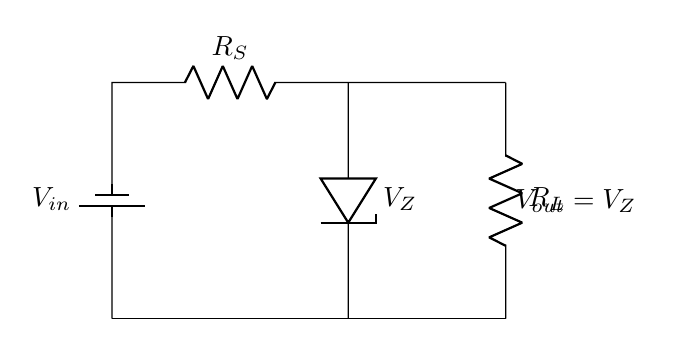
\begin{tikzpicture}
    \draw (0,0) to[battery1, l=$V_{in}$] (0,3) to[R, l=$R_S$] (3,3) -- (5,3);
    \draw (3,3) to[zD, l=$V_Z$] (3,0);
    \draw (5,3) to[R, l=$R_L$] (5,0);
    \draw (0,0) -- (5,0);
    
    \node[right] at (5, 1.5) {$V_{out} = V_Z$};
\end{tikzpicture}
\captionof{figure}{Zener Voltage Regulator}
\end{center}

\textbf{Working Principle:}

\begin{itemize}
    \item \keyword{Normal operation}: Zener diode is reverse biased and conducts when voltage reaches breakdown voltage
    \item \keyword{Voltage regulation}: When input voltage rises, more current flows through Zener diode, maintaining constant voltage across it
    \item \keyword{Load variation}: When load draws more current, less current flows through Zener, keeping voltage stable
    \item \keyword{Series resistor}: Limits current and drops excess voltage
\end{itemize}

\textbf{Circuit behavior:}
\begin{itemize}
    \item $V_{out} = V_z$ (Zener breakdown voltage)
    \item $I_z = (V_{in} - V_z)/R - I_L$
\end{itemize}
\end{solutionbox}

\begin{mnemonicbox}
\mnemonic{SERZ: "Series resistor Enables Regulation with Zener"}
\end{mnemonicbox}

\questionmarks{3(c) OR}{7}{Explain V-I char of P-N junction diode and give comparison between P-N junction diode and Zener diode.}

\begin{solutionbox}
\textbf{Answer}:

\textbf{V-I Characteristics of P-N Junction Diode:}

\begin{center}
\begin{tikzpicture}
    \draw[->] (-3,0) -- (3,0) node[right] {$V$};
    \draw[->] (0,-3) -- (0,3) node[above] {$I$};
    
    % Forward
    \draw[thick, blue] (0,0) -- (0.7,0) .. controls (0.8,0.1) and (0.9,1) .. (1,2.5);
    \node at (1.5, 1) {Forward};
    
    % Reverse
    \draw[thick, red] (0,0) -- (-2,0) -- (-2,-2.5);
    \node[below] at (-2,0) {Breakdown};
    \node[left] at (-1, -1) {Reverse};
\end{tikzpicture}
\captionof{figure}{Diode V-I Characteristics}
\end{center}

\textbf{Key Points:}
\begin{itemize}
    \item \keyword{Forward bias}: Conducts easily after exceeding knee voltage ($\approx 0.7V$ for silicon)
    \item \keyword{Reverse bias}: Very small leakage current until breakdown voltage
    \item \keyword{Breakdown region}: Occurs at high reverse voltage, causes damage in normal diodes
\end{itemize}

\textbf{P-N Junction Diode vs. Zener Diode:}

\begin{center}
\captionof{table}{Comparison P-N vs Zener}
\begin{tabulary}{\linewidth}{|L|L|L|}
\hline
\textbf{Parameter} & \textbf{P-N Junction Diode} & \textbf{Zener Diode} \\ \hline
\textbf{Symbol} & Standard Diode Symbol & Z-Symbol Diode \\ \hline
\textbf{Forward operation} & Conducts easily & Same as normal diode \\ \hline
\textbf{Reverse breakdown} & At high voltage, causes damage & Controlled, non-destructive \\ \hline
\textbf{Doping level} & Moderate & Heavily doped \\ \hline
\textbf{Operating region} & Forward biased & Reverse biased (breakdown region) \\ \hline
\textbf{Applications} & Rectification, switching & Voltage regulation, reference \\ \hline
\textbf{Breakdown mechanism} & Avalanche & Zener effect and avalanche \\ \hline
\textbf{Temperature coefficient} & Negative & Can be positive or negative \\ \hline
\end{tabulary}
\end{center}
\end{solutionbox}

\begin{mnemonicbox}
\mnemonic{FORD: "Forward Operation for Rectifiers, Diodes; reverse operation for Zeners"}
\end{mnemonicbox}

\questionmarks{4(a)}{3}{Describe working principle of Photodiode.}

\begin{solutionbox}
\textbf{Answer}:

\textbf{Working Principle of Photodiode:}

\begin{center}
\begin{tikzpicture}[node distance=2cm]
    \node [gtu block, fill=lightyellow] (light) {Light};
    \node [gtu block, fill=lightpink, right=of light] (pn) {P-N Junction};
    \node [gtu block, fill=lightblue, right=of pn] (eh) {Electron-Hole Pairs};
    \node [gtu block, fill=lightgreen, right=of eh] (curr) {Photocurrent};
    
    \draw [gtu arrow] (light) -- (pn);
    \draw [gtu arrow] (pn) -- (eh);
    \draw [gtu arrow] (eh) -- (curr);
\end{tikzpicture}
\captionof{figure}{Photodiode Flow}
\end{center}

\begin{itemize}
    \item \keyword{Construction}: P-N junction diode with transparent window or lens
    \item \keyword{Operation}: Reverse biased operation for light detection
    \item \keyword{Photon absorption}: Incoming photons create electron-hole pairs in depletion region
    \item \keyword{Current generation}: Electric field sweeps carriers to respective terminals, creating photocurrent
    \item \keyword{Light sensitivity}: Current proportional to light intensity
\end{itemize}
\end{solutionbox}

\begin{mnemonicbox}
\mnemonic{LIGER: "Light Induces Generation of Electrons in Reverse-bias"}
\end{mnemonicbox}

\questionmarks{4(b)}{4}{Explain the characteristic of Schottky barrier diode.}

\begin{solutionbox}
\textbf{Answer}:

\textbf{Schottky Barrier Diode Characteristics:}

\begin{center}
\begin{tikzpicture}
    \draw[->] (-2,0) -- (3,0) node[right] {$V$};
    \draw[->] (0,-2) -- (0,3) node[above] {$I$};
    
    \draw[thick, red] (0,0) -- (0.3,0) .. controls (0.4,0.1) and (0.5,1) .. (0.6,2.5);
    \node[left] at (0.6, 2) {Schottky};
    
    \draw[thick, blue, dashed] (0,0) -- (0.7,0) .. controls (0.8,0.1) and (0.9,1) .. (1,2.5);
    \node[right] at (1, 1.5) {PN Junction};
\end{tikzpicture}
\captionof{figure}{Schottky vs PN Junction}
\end{center}

\begin{itemize}
    \item \keyword{Low forward voltage drop}: 0.2-0.3V compared to 0.7V for silicon PN junction
    \item \keyword{Fast switching}: No minority carrier storage, minimal reverse recovery time
    \item \keyword{Construction}: Metal-semiconductor junction instead of P-N junction
    \item \keyword{No reverse recovery time}: Majority carrier device (no stored charge)
    \item \keyword{Applications}: High-frequency applications, rectifiers in power supplies
\end{itemize}
\end{solutionbox}

\begin{mnemonicbox}
\mnemonic{FAST: "Forward voltage low, Allows Switching Timely"}
\end{mnemonicbox}

\questionmarks{4(c)}{7}{Explain working principle of PNP and NPN transistor.}

\begin{solutionbox}
\textbf{Answer}:

\textbf{NPN Transistor Structure and Working:}

\begin{center}
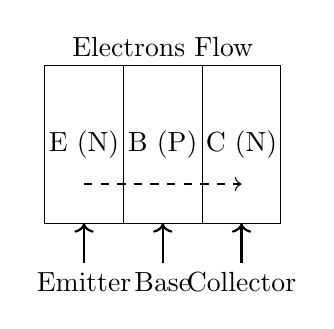
\begin{tikzpicture}
    \draw (0,0) rectangle (3,2);
    \draw (1,0) -- (1,2);
    \draw (2,0) -- (2,2);
    \node at (0.5, 1) {E (N)};
    \node at (1.5, 1) {B (P)};
    \node at (2.5, 1) {C (N)};
    
    \draw[->, thick] (0.5, -0.5) -- (0.5, 0); % Emitter connection
    \draw[->, thick] (1.5, -0.5) -- (1.5, 0); 
    \draw[->, thick] (2.5, -0.5) -- (2.5, 0);
    
    \node[below] at (0.5, -0.5) {Emitter};
    \node[below] at (1.5, -0.5) {Base};
    \node[below] at (2.5, -0.5) {Collector};
    
    \draw[->, dashed] (0.5, 0.5) -- (2.5, 0.5);
    \node[above] at (1.5, 2) {Electrons Flow};
\end{tikzpicture}
\captionof{figure}{NPN Structure}
\end{center}

\begin{itemize}
    \item \keyword{Biasing}: Emitter-base junction forward biased, collector-base junction reverse biased
    \item \keyword{Current flow}: Electrons from emitter to collector through thin base region
    \item \keyword{Amplification principle}: Small base current controls larger collector current
    \item \keyword{Current relationship}: $I_E = I_B + I_C$
    \item \keyword{Majority carriers}: Electrons
\end{itemize}

\textbf{PNP Transistor Structure and Working:}

\begin{itemize}
    \item \keyword{Biasing}: Emitter-base junction forward biased, collector-base junction reverse biased
    \item \keyword{Current flow}: Holes from emitter to collector through thin base region
    \item \keyword{Amplification principle}: Small base current controls larger collector current
    \item \keyword{Current relationship}: $I_E = I_B + I_C$
    \item \keyword{Majority carriers}: Holes
    \item \keyword{Current direction}: Opposite to NPN (conventional current from emitter to collector)
\end{itemize}
\end{solutionbox}

\begin{mnemonicbox}
\mnemonic{NPNP: "Negative carriers in NPN, Positive carriers in PNP"}
\end{mnemonicbox}

\questionmarks{4(a) OR}{3}{Describe working principle of LED.}

\begin{solutionbox}
\textbf{Answer}:

\textbf{Working Principle of LED:}

\begin{center}
\begin{tikzpicture}[node distance=2cm]
    \node [gtu block, fill=lightblue] (bias) {Forward Bias};
    \node [gtu block, fill=lightpink, right=of bias] (recomb) {e-h Recombination};
    \node [gtu block, fill=lightyellow, right=of recomb] (energy) {Energy Release};
    \node [gtu block, fill=lightgreen, right=of energy] (light) {Light};
    
    \draw [gtu arrow] (bias) -- (recomb);
    \draw [gtu arrow] (recomb) -- (energy);
    \draw [gtu arrow] (energy) -- (light);
\end{tikzpicture}
\captionof{figure}{LED Principle}
\end{center}

\begin{itemize}
    \item \keyword{Construction}: P-N junction made from direct bandgap semiconductor materials
    \item \keyword{Forward biasing}: Electrons from n-region and holes from p-region recombine at junction
    \item \keyword{Recombination}: Electrons fall from conduction band to valence band
    \item \keyword{Energy emission}: Energy released during recombination emits photons (light)
\end{itemize}
\end{solutionbox}

\begin{mnemonicbox}
\mnemonic{REBEL: "Recombination of Electrons and holes By Energetic Light emission"}
\end{mnemonicbox}

\questionmarks{4(b) OR}{4}{Explain function of transistor as switch in cut off and application of saturation region.}

\begin{solutionbox}
\textbf{Answer}:

\textbf{Transistor as a Switch:}

\begin{center}
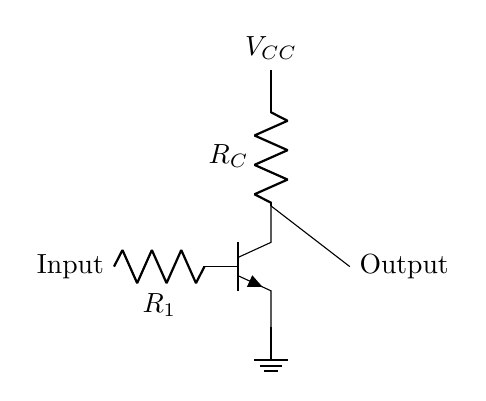
\begin{tikzpicture}
    \draw (0,0) node[npn] (Q) {};
    \draw (Q.E) node[ground] {};
    \draw (Q.C) to[R, l=$R_C$] (0,2) -- (0,2.5) node[above] {$V_{CC}$};
    \draw (Q.B) to[R, l=$R_1$] (-2,0) node[left] {Input};
    \draw (Q.C) -- (1,0) node[right] {Output};
\end{tikzpicture}
\captionof{figure}{Transistor Switch Circuit}
\end{center}

\textbf{Cut-off Region (Switch OFF):}
\begin{itemize}
    \item \keyword{Base voltage}: Below 0.7V (for silicon)
    \item \keyword{Base current}: Approximately zero
    \item \keyword{Collector current}: Approximately zero
    \item \keyword{Collector-emitter voltage}: Equal to supply voltage
    \item \keyword{Applications}: Logic gates, digital circuits, relay drivers
\end{itemize}

\textbf{Saturation Region (Switch ON):}
\begin{itemize}
    \item \keyword{Base voltage}: Well above 0.7V
    \item \keyword{Base current}: Sufficient to ensure minimum $V_{CE}$
    \item \keyword{Collector current}: Maximum (limited by collector resistor)
    \item \keyword{Collector-emitter voltage}: Very low (0.2V - 0.3V)
    \item \keyword{Applications}: Digital switches, motor drivers, LED drivers
\end{itemize}
\end{solutionbox}

\begin{mnemonicbox}
\mnemonic{COSI: "Cutoff Opens Switch, Input saturates to close"}
\end{mnemonicbox}

\questionmarks{4(c) OR}{7}{Explain common emitter (CE) configuration of Transistor. Derive relation between α and β for transistor amplifier.}

\begin{solutionbox}
\textbf{Answer}:

\textbf{Common Emitter Configuration:}

\begin{center}
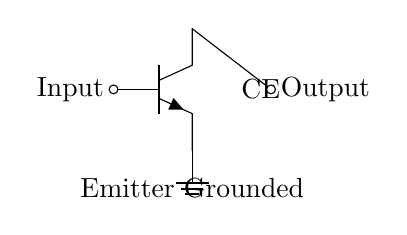
\begin{tikzpicture}
    \draw (0,0) node[npn] (Q) {};
    \node [right=0.5cm of Q] {CE};
    \draw (Q.E) node[ground] {};
    \draw (Q.B) to[short,-o] (-1,0) node[left] {Input};
    \draw (Q.C) to[short,-o] (1,0) node[right] {Output};
    \node[below] at (0,-1) {Emitter Grounded};
\end{tikzpicture}
\captionof{figure}{CE Configuration}
\end{center}

\textbf{Characteristics:}
\begin{itemize}
    \item \keyword{Input/Output}: Base / Collector
    \item \keyword{Gains}: High Current ($\beta$), High Voltage
    \item \keyword{Impedance}: Medium Input, High Output
\end{itemize}

\textbf{Relationship between $\alpha$ and $\beta$:}

By definition:
\begin{itemize}
    \item $\alpha = I_C/I_E$
    \item $\beta = I_C/I_B$
\end{itemize}

From Kirchhoff's Current Law:
\[ I_E = I_B + I_C \]

Dividing by $I_E$:
\[ 1 = \frac{I_B}{I_E} + \frac{I_C}{I_E} = \frac{I_B}{I_E} + \alpha \]
\[ \frac{I_B}{I_E} = 1 - \alpha \]

Now, 
\[ \beta = \frac{I_C}{I_B} = \frac{I_C/I_E}{I_B/I_E} = \frac{\alpha}{1-\alpha} \]
\end{solutionbox}

\begin{mnemonicbox}
\mnemonic{BEAR: "Beta Equals Alpha divided by (1-alpha) Relation"}
\end{mnemonicbox}

\questionmarks{5(a)}{3}{What do you mean by E-waste? What are the different methods of E-waste disposal?}

\begin{solutionbox}
\textbf{Answer}:

\textbf{E-waste (Electronic Waste)}: Discarded electronic devices and components that have reached end of life or are no longer useful.

\textbf{Methods of E-waste Disposal:}

\begin{center}
\captionof{table}{Disposal Methods}
\begin{tabulary}{\linewidth}{|L|L|}
\hline
\textbf{Disposal Method} & \textbf{Description} \\ \hline
\textbf{Recycling} & Separating valuable materials like metals, plastics for reuse \\ \hline
\textbf{Landfilling} & Disposing in designated landfills (not recommended) \\ \hline
\textbf{Incineration} & Burning waste at high temperatures (creates toxic emissions) \\ \hline
\textbf{Reuse/Refurbishment} & Repairing and upgrading for extended use \\ \hline
\textbf{Extended Producer Responsibility} & Manufacturers take back and handle disposal \\ \hline
\end{tabulary}
\end{center}
\end{solutionbox}

\begin{mnemonicbox}
\mnemonic{RIPER: "Recycling Is Preferable to Environmentally-harmful Remedies"}
\end{mnemonicbox}

\questionmarks{5(b)}{4}{Explain methods of handling electronic waste with examples.}

\begin{solutionbox}
\textbf{Answer}:

\textbf{Methods of Handling Electronic Waste:}

\begin{center}
\begin{tikzpicture}[node distance=1.5cm]
    \node [gtu block] (coll) {Collection};
    \node [gtu block, right=of coll] (sort) {Sorting};
    \node [gtu block, right=of sort] (dism) {Dismantling};
    \node [gtu block, below=of dism] (recov) {Recovery};
    \node [gtu block, left=of recov] (disp) {Disposal};
    
    \draw [gtu arrow] (coll) -- (sort);
    \draw [gtu arrow] (sort) -- (dism);
    \draw [gtu arrow] (dism) -- (recov);
    \draw [gtu arrow] (recov) -- (disp);
\end{tikzpicture}
\captionof{figure}{E-waste Handling Flow}
\end{center}

\begin{itemize}
    \item \keyword{Collection and Segregation}: Dedicated bins, prevents mixing (e.g., e-waste bins).
    \item \keyword{Dismantling and Resource Recovery}: Recovering gold/copper from PCBs.
    \item \keyword{Refurbishment and Reuse}: Repairing old computers.
    \item \keyword{Proper Disposal}: Specialized treatment for hazardous parts (mercury).
\end{itemize}
\end{solutionbox}

\begin{mnemonicbox}
\mnemonic{CREED: "Collect, Recover, Extract, Extend, Dispose safely"}
\end{mnemonicbox}

\questionmarks{5(c)}{7}{What is ripple factor? Derive the equation of the ripple factor for rectifier.}

\begin{solutionbox}
\textbf{Answer}:

\textbf{Ripple Factor}: Ratio of RMS value of AC component to DC component in the output ($\gamma = V_{AC}/V_{DC}$).

\textbf{Derivation for Half Wave Rectifier:}

Assume $v = V_m\sin\omega t$.

\textbf{Step 1}: Find DC component (average value)
\[ V_{DC} = \frac{1}{2\pi} \int_{0}^{\pi} V_m\sin\omega t \, d(\omega t) = \frac{V_m}{\pi} \]

\textbf{Step 2}: Find RMS value
\[ V_{RMS} = \sqrt{\frac{1}{2\pi} \int_{0}^{\pi} V_m^2\sin^2\omega t \, d(\omega t)} = \frac{V_m}{2} \]

\textbf{Step 3}: Find AC component
\[ V_{AC} = \sqrt{V_{RMS}^2 - V_{DC}^2} = \sqrt{\left(\frac{V_m}{2}\right)^2 - \left(\frac{V_m}{\pi}\right)^2} \]

\textbf{Step 4}: Calculate ripple factor
\[ \gamma = \frac{V_{AC}}{V_{DC}} = \frac{\sqrt{V_{RMS}^2 - V_{DC}^2}}{V_{DC}} = \sqrt{\left(\frac{V_{RMS}}{V_{DC}}\right)^2 - 1} \]
\[ \gamma = \sqrt{\left(\frac{V_m/2}{V_m/\pi}\right)^2 - 1} = \sqrt{\left(\frac{\pi}{2}\right)^2 - 1} = \sqrt{1.57^2 - 1} = 1.21 \]

For Full Wave Rectifier, $\gamma = 0.48$.
\end{solutionbox}

\begin{mnemonicbox}
\mnemonic{ROAD: "Ripple is Output's AC Divided by DC component"}
\end{mnemonicbox}

\questionmarks{5(a) OR}{3}{Which are the toxic substances present in e-waste?}

\begin{solutionbox}
\textbf{Answer}:

\begin{center}
\captionof{table}{Toxic Substances in E-waste}
\begin{tabulary}{\linewidth}{|L|L|L|}
\hline
\textbf{Toxic Substance} & \textbf{Source} & \textbf{Impact} \\ \hline
\textbf{Lead (Pb)} & Solder, CRT, batteries & Neurological damage \\ \hline
\textbf{Mercury (Hg)} & Switches, backlights & Kidney damage \\ \hline
\textbf{Cadmium (Cd)} & Batteries, PCBs & Bone disease \\ \hline
\textbf{Flame Retardants} & Plastics & Endocrine disruption \\ \hline
\textbf{Beryllium (Be)} & Connectors & Lung disease \\ \hline
\end{tabulary}
\end{center}
\end{solutionbox}

\begin{mnemonicbox}
\mnemonic{LMBCHB: "Lead, Mercury, and Beryllium Cause Harmful Bodily effects"}
\end{mnemonicbox}

\questionmarks{5(b) OR}{4}{Write important parameters for selecting the right transistor for your application and explain any two.}

\begin{solutionbox}
\textbf{Answer}:

\textbf{Selection Parameters:}
\begin{itemize}
    \item Maximum collector current ($I_C$)
    \item Maximum collector-emitter voltage ($V_{CEO}$)
    \item Current gain ($h_{FE}$ or $\beta$)
    \item Power dissipation ($P_{tot}$)
\end{itemize}

\textbf{Maximum Collector Current ($I_C$):}
\begin{itemize}
    \item Maximum current that can flow through collector without damage.
    \item Must exceed application's peak requirement.
\end{itemize}

\textbf{Current Gain ($\beta$):}
\begin{itemize}
    \item Ratio of collector current to base current.
    \item Determines amplification capability; high gain needed for switching to reduce base drive.
\end{itemize}
\end{solutionbox}

\begin{mnemonicbox}
\mnemonic{GIVE: "Gain and Ic are Very Essential parameters"}
\end{mnemonicbox}

\questionmarks{5(c) OR}{7}{What is rectifier efficiency? Find out efficiency of the full wave rectifier.}

\begin{solutionbox}
\textbf{Answer}:

\textbf{Rectifier Efficiency ($\eta$)}: Ratio of DC output power to AC input power ($\eta = P_{DC}/P_{AC} \times 100\%$).

\textbf{Derivation for Full Wave Rectifier:}

\textbf{Step 1}: Calculate DC output power
\[ V_{DC} = \frac{2V_m}{\pi}, \quad I_{DC} = \frac{V_{DC}}{R_L} \]
\[ P_{DC} = I_{DC}^2 R_L = \frac{4V_m^2}{\pi^2 R_L} \]

\textbf{Step 2}: Calculate AC input power
\[ V_{RMS} = \frac{V_m}{\sqrt{2}}, \quad I_{RMS} = \frac{V_{RMS}}{R_L} \]
\[ P_{AC} = I_{RMS}^2 R_L = \frac{V_m^2}{2R_L} \]

\textbf{Step 3}: Calculate efficiency
\[ \eta = \frac{P_{DC}}{P_{AC}} = \frac{4V_m^2 / (\pi^2 R_L)}{V_m^2 / (2R_L)} = \frac{8}{\pi^2} \]
\[ \eta = \frac{8}{9.87} \approx 0.812 = 81.2\% \]

\textbf{Comparison:}
\begin{itemize}
    \item Half Wave: 40.6\%
    \item Full Wave: 81.2\%
\end{itemize}
\end{solutionbox}

\begin{mnemonicbox}
\mnemonic{PIDE: "Power Input Determines Efficiency"}
\end{mnemonicbox}

\end{document}
